\chapter{Background Estimation}
\label{ch:6}

% **************************** Define Graphics Path **************************
\ifpdf
    \graphicspath{{Chapter6/Figs/Raster/}{Chapter6/Figs/PDF/}{Chapter6/Figs/}}
\else
    \graphicspath{{Chapter6/Figs/Vector/}{Chapter6/Figs/}}
\fi

Maybe some stuff here introducing the chapter...

%********************************** % First Section  *************************************
\section{Overview of TF method}  %Section - 1.1 
\label{sec:background_overview}

Contributions from Standard Model background processes are estimated using a data-driven 
prediction technique, employing dedicated control samples. A transfer factor (TF) 
is used, constructed from MC samples as the ratio 
of the MC yield in the signal region, \\$N_{MC}^{signal}\big(\HT, \nj, \nb\big)$,
and the MC yield of a given control region, \\$N_{Data}^{control}\big(\HT, \nj, \nb\big)$,
as a function of the analysis binning, \HT, \nj and \nb, as shown by
equation~\ref{eq:transfer_factor}.

\begin{equation}
TF = \frac{N_{MC}^{signal}\big(\HT, \nj, \nb\big)}{N_{MC}^{control}\big(\HT, \nj, \nb\big)}
\label{eq:transfer_factor}
\end{equation}

For a given \HT, \nj and \nb bin, the TF is used to extrapolate a yield in data from
the control region, $N_{Data}^{control}\big(\HT, \nj, \nb\big)$
to the signal region $N_{Data}^{signal}\big(\HT, \nj, \nb\big)$, as shown in
equation~\ref{eq:transfer_equation}.

\begin{equation}
N_{Data}^{signal}\big(\HT, \nj, \nb\big) = N_{Data}^{control}\big(\HT, \nj, \nb\big)
\times TF
\label{eq:transfer_equation}
\end{equation}

The control samples are statistically independent and each used for predicting 
specific background processes, the details of which are described in 
the following section, section~\ref{sec:background_control}.

To construct the MC yields, the following process-specific samples are considered:
W + jets (\numw),
\ttbar + jets (\numtt), DY + jets (\numdy), $\gamma$ + jets(\numgam),
single top + jets (\numtop), WW + jets, WZ + jets and ZZ + jets (\numdibo), and
\zinv + jets (\numzinv).

The predictions made using this technique alone are considered as ``na\"{i}ve'' 
predictions and are only used in analysis development and the derivation of 
background systematics. In order to determine final yields for use in interpretation and 
limit-setting, a fit is made across all signal and control regions, using the 
full likelihood model, as described later in chapter~REF. For this, the derived 
transfer factors and individual yields enter as terms in the likelihood, where 
all related systematics, potential correlations and signal contamination are
accounted for in the fit. 

The denominator of each transfer factor is constructed using the sum of all MC
sample yields, for a given control region and category:

\begin{equation}
N_{MC}^{control}\big(\HT, \nj, \nb\big) = \numw + \numtt + \numdy + \numgam + 
\numtop + \numdibo + \numzinv
\label{eq:trans_fact_denom}
\end{equation}

The numerator is constructed according to the b-tag mutliplicity being 
considered. For $\nb \leq 1$, the \mj control region is used to predict 
predominantly \ttbar + jets and W + jets, however an estimate for all other 
residual backgrounds is produced. All MC samples are used with the exception of
\zinv:

\begin{equation}
N_{MC}^{signal}\big(\HT, \nj, \nb \leq 1\big) = \numw + \numtt + \numdy + \numgam + 
\numtop + \numdibo
\label{eq:trans_fact_num_le1b_noz}
\end{equation}

The \zinv + jets component of the background is predicted using the \mmj
and \gj control samples, using only the \zinv MC yields:

\begin{equation}
N_{MC}^{signal}\big(\HT, \nj, \nb \leq 1 \big) = \numzinv
\label{eq:trans_fact_num_le1b_z}
\end{equation}

Again, it should be noted here that although two seperate control samples are 
used to estimate the \zinv background contribution, the result of each
considered by the global fit used to produce the final background prediction.

For $\nb \geq 2$, the \mj sample is used to produce a prediction for all 
SM processes, including \zinv, and therefore the numerator of the TF is defined as:

\begin{equation}
N_{MC}^{signal}\big(\HT, \nj, \nb \geq 2 \big) = \numw + \numtt + \numdy + \numgam + 
\numtop + \numdibo + \numzinv
\label{eq:trans_fact_num_geq2b}
\end{equation}

The \mmj and \gj control samples are not used beyond the $\nb \leq 1$ categories
due to the statistical limitations of such samples at high b-tag multiplicities.
A full summary of the control regions used for predictions per analysis category
is shown in table~\ref{tab:control_prediction_summary}.

\begin{table}[h!]
  \caption{Summary of control samples used to predict the SM
    background for each event category. REWORD}
  \label{tab:control_prediction_summary}
  \centering
  \begin{tabular}{ lll }
    \hline
    \hline
    \nj     & \nb     & Control samples \\ [1.0ex]
    \hline
    2--3    & 0       & \mj, \mmj, \gj  \\
    2--3    & 1       & \mj, \mmj, \gj  \\
    2--3    & 2       & \mj             \\
    $\geq$4 & 0       & \mj, \mmj, \gj  \\
    $\geq$4 & 1       & \mj, \mmj, \gj  \\
    $\geq$4 & 2       & \mj             \\
    $\geq$4 & 3       & \mj             \\
    $\geq$4 & $\geq4$ & \mj             \\
    \hline
    \hline
  \end{tabular}
\end{table}

By employing a technique that uses a ratio of MC yields, reliance on MC is 
greatly reduced. Errors inherent to MC samples, such as mismodelling effects, 
will cancel in the ratio. These errors can potentially include kinematic
mismodelling, which would affect analysis acceptance, and mismodelling of 
instrumental effects, which could have an affect on object 
reconstruction efficiencies. However, any remaining systematics such as these
and others 
are probed using Closure Tests (CT), described in detail in a later section REF.


%********************************** % Second Section  *************************************
\section{Control samples}  %Section - 1.2
\label{sec:background_control}

Control sample definitions are designed such that they are as close as possible 
to that of the signal region, with the exception of a selected `tag' muon or 
photon, which is subsequently ignored for the calculation of all analysis 
variables, such as \HT, \met, \alphat etc. Other differences include mass-window
and minor kinematic cuts, used to enrich the control samples in certain processes. 
The samples themselves are statistically independent, and orthogonal to the 
signal region due to the selection of the tagged lepton or photon minimising any 
possible signal contamination. However, a full treatment of the
signal-contamination and sample cross-correlation is taken into account in the
background fit and final limit-setting. 

This section will describe the main control regions in more detail, including 
their targetted background estimations, selection cuts specific to each and their
trigger requirements.

\subsection{mu + jets}

The \mj control sample is constructed by selecting a single muon with associated 
jets. This region is used to predict backgrounds from processes such as \wj and
\ttj. This covers not only the leptonic decays of such productions, where the 
lepton is unidentified for whatever reason, but also the hadronic decays of tau 
leptons [from high-\Pt W bosons]. The event selection therefore is optimised to 
select W bosons decaying to a muon and a neutrino in the phase-space of the 
signal.

\subsubsection{Triggers}
\label{sec:mujets_control_trigger}
Events are collected using the loosely-isolated, $\eta$-restricted
\verb!HLT_IsoMu24_eta2p1! trigger, which was in place throughout the 8\tev
data-taking period. The efficiency of this trigger was measured by the muon POG 
using a tag-and-probe method [REF], in bins of the muon \Pt and $\eta$, as summarised 
in table~\ref{tab:muon-trig-effs}. [mention non-dependency on HT?]

\begin{table}[!h]
  \caption{Muon trigger efficiencies (\%). Statistical uncertainties
    are at the per-mille level, while a relative systematic
    uncertainty on all measurements is assumed to be 1\%. REWORD}
  \label{tab:muon-trig-effs}
  \centering
  \footnotesize
  \begin{tabular}{ cccc }
    \hline
    \hline
    \HT (GeV) & 2-3 & $\geq$4 \\ [0.5ex]
    \hline
%    200--275  & 89.1 & 89.8  \\
%    275--325  & 89.3 & 89.8  \\
%    325--375  & 89.5 & 90.0  \\
%    375--475  & 89.7 & 90.3  \\
%    475--575  & 89.8 & 90.5  \\
%    575--675  & 90.0 & 90.6  \\
%    675--775  & 90.1 & 90.7  \\
%    775--875  & 90.2 & 90.8  \\
%    875--975  & 90.4 & 90.6  \\
%    975--1075 & 90.3 & 90.6  \\
%    $>$1075   & 90.0 & 91.2  \\
    150--200  & 87.2 & 88.1  \\
    200--275  & 87.5 & 88.1  \\
    275--325  & 87.8 & 88.2  \\
    325--375  & 87.9 & 88.4  \\
    375--475  & 88.1 & 88.6  \\
    475--575  & 88.2 & 88.8  \\
    575--675  & 88.4 & 88.9  \\
    675--775  & 88.5 & 89.0  \\
    775--875  & 88.6 & 89.1  \\
    875--975  & 88.8 & 89.0  \\
    975--1075 & 88.7 & 89.0  \\
    $>$1075   & 88.4 & 89.6  \\
    \hline
    \hline
  \end{tabular}
\end{table}

\subsubsection{Selection Criteria}
\label{sec:mujets_control_selection}
A single tight isolated muon is selected, with \Pt > 30\gev and $|\eta| <$2.1, 
with the thresholds chosen due to trigger requirements. The transverse mass
of the W, reconstructed by the 
$\mu$ and the \met (originating from the $\nu_{\mu}$), is required to be in a 
loose window around $m_W$, $30 < M(\mu, \met) < 125\gev$, in order to surpress 
QCD mutlijet contributions. Events are vetoed if $\Delta R(\mu, jet_{i}) < 0.5$,
for all jets $i$ in the event. To keep the selection as close to the signal 
region as possible, other cuts such as the single isolated track veto and 
\mhtmet cuts are also applied.

Specifically for the \mj (and \mmj) control samples, no \alphat requirement is
made in order to increase the statistics and therefore the predictive power of 
the samples. This is possible as the other requirements, in particular the 
requirement of
a single muon and a specific invariant mass window, greatly reduce any potential
contamination from QCD MJ events. The ability to do this is specifically tested, 
in a dedicated closure test as described later in section~\ref{sec:closure_tests}.

\subsection{mumu + jets}
The \mmj sample is constructed to predict background contributions from \zinv 
decays, mimicking this decay via the $Z\to\mu\mu + jets$ process where both 
muons are subsequently ignored, which is kinematically very similar.
The sample is used to provide low \HT coverage for the \zinv background 
prediction, where the \gj sample is unable to do so.

\subsubsection{Triggers}
The trigger used is the same as for the \mj sample, as described in
section~\ref{sec:mujets_control_trigger}. For the dimuon selection, however, 
trigger efficiencies are slightly improved given that either of the muons 
present can cause the positive trigger decision. The trigger efficiencies
for the \mmj selection are summarised in table~\ref{tab:dimuon-trig-effs}.

\begin{table}[!h]
  \caption{Muon trigger efficiencies (\%). Statistical uncertainties
    are at the per-mille level, while a relative systematic
    uncertainty on all measurements is assumed to be 1\%. REWORD}
  \label{tab:dimuon-trig-effs}
  \centering
  \footnotesize
  \begin{tabular}{ cccc }
    \hline
    \hline
    \HT (GeV) & 2-3 & $\geq$4 \\ [0.5ex]
                                       
    \hline
    150--200  & 98.4 & 98.4  \\
    200--275  & 98.5 & 98.4  \\
    275--325  & 98.5 & 98.4  \\
    325--375  & 98.6 & 98.6  \\
    375--475  & 98.6 & 98.5  \\
    475--575  & 98.6 & 98.6  \\
    575--675  & 98.6 & 98.6  \\
    675--775  & 98.7 & 98.6  \\
    775--875  & 98.6 & 98.6  \\
    875--975  & 98.7 & 98.6  \\
    975--1075 & 98.7 & 98.8  \\
    $>$1075   & 98.7 & 98.7  \\
    \hline
    \hline
  \end{tabular}
\end{table}

\subsubsection{Selection Criteria}
The selection for the \mmj sample is very similar to that of the \mj sample, 
described in section~\ref{sec:mujets_control_selection}, with differences chosen
to enrich the sample in Z bosons decaying to pairs of muons in the kinematic 
phase space of the signal region. Two tight isolated muons are selected, each 
with $\Pt > 30\gev$ and $|\eta| < 2.1$, and their invariant mass is chosen to be
tight around $m_Z$, $m_Z - 25 < M_{\mu_1\mu_2} < m_Z + 25 \gev$. Furthermore, a 
veto is made on events satisfying $\Delta R(\mu_i, jet_j) < 0.5$, for every muon 
$i$ and every jet $j$. Similarly as in the \mj sample selection, no \alphat
requirement is made.

\subsection{photon + jets}
The \gj sample is used to predict the \zinv background contribution, given it's 
similar kinematics when the $\gamma$ is ignored from the event, and larger 
production cross section relative to \mmj. Given the trigger thresholds, the \gj
sample cannot make predictions for $\HT<375\gev$, and so is complimentarily used
alongside the \mmj sample prediction.

\subsubsection{Triggers}
Events are collected using the \verb!HLT_Photon150! trigger. The trigger's 
efficiency is measured using the \verb!HLT_Photon90! trigger as a reference, and
is found to be 100$\%$ efficient for $E_T^{photon}>165\gev$ and $\HT>375\gev$, 
as shown by the turn on curves in figure~

\begin{figure}[ht!]
  \centering
  \begin{subfigure}[b]{0.48\textwidth}
    \includegraphics[width=\textwidth, page=3,trim=40 50 160 120,clip=true]{figures/trigger/g_barrel_375_caloJet_le3j.pdf}
    \caption{\njlow}
    \label{fig:photon_control_trigeff_le3j}
  \end{subfigure}
  \begin{subfigure}[b]{0.48\textwidth}
    \includegraphics[width=\textwidth, page=3,trim=40 50 160 120,clip=true]{figures/trigger/g_barrel_375_caloJet_ge4j.pdf}
    \caption{\njhigh}
    \label{fig:photon_control_trigeff_ge4j}
  \end{subfigure}
  \caption{Efficiency turn-on curves for
      the photon trigger that records events that
      satisfy the \gj selection criteria, $E_{T}^{photon} > 165\gev$, $\HT > 375\gev$, and \njlow (Left) and \njhigh
      (Right). REWORD}
  \label{fig:photon_control_trigeff}
\end{figure}

\subsubsection{Selection Criteria}
Exactly one photon satisying tight isolation criteria is required, with 
$\Pt > 165\gev$ and $|\eta|<1.45$. In addition, events are vetoed if
$\Delta R(\gamma, jet_i)<1.0$ is satisfied, for all of the events $i$ jets.


\subsection{jets}
Overview
Targetted backgrounds
\subsubsection{Triggers}
\subsubsection{Selection Criteria}

\subsection{HT sideband normalisation}
As mentioned previously in section~\ref{sec:mc_xsec_corrs}, absolute MC 
normalisation has always been mis-modelled in the high-\met (CHECK) region of 
phase-space that SUSY analyses tend to search in. As such, data and MC appear to
disagree using `out-of-the-box' MC samples and cross-sections. While data and MC
comparisons are not explicitly used in this analysis, ratios of MC yields are, 
and so a sideband in \HT is used to extract a cross-section correction factor for the main 
MC processes. Correction factors are determined as the data to MC ratio in the $
150 \leq \HT < 200 \gev$ sideband region, in a given control sample with a 
given selection, designed to produce a pure sample of a background process. A
summary of the selections and their relevant purities is given in table~\ref{tab:ht_sideband}.

\begin{table}[!ht]
  \caption{Correction factors determined from a data sideband for the different
    MC samples. All Correction factors are relative to theoretical cross
    sections calculated at NNLO. The corrections measured for the W +
    jets and Z + jets processes, which are in agreement, are also
    applied to the \zinv + jets and \gj samples. ``Corrected yield''
    reflects the observed data yield minus the contamination as given
    by MC. REWORD}
  \label{tab:ht_sideband}
  \centering
  \scriptsize
  \begin{tabular}{ llcccc }
    \hline
    \hline
    Process                       & Selection                         & Purity & Corrected yield & MC expectation      & Correction factor        \\
    \hline
    W + jets                      & \mj, \njlow, $\nb = 0$          & 0.91   & 25737           & $27529.0 \pm 350.7$ & $0.93 \pm 0.01$ \\
    Z($\rightarrow\mu\mu$) + jets & \mmj, \njlow, $\nb = 0$         & 0.98   & 1826            & $1947.3 \pm 59.5$   & $0.94 \pm 0.04$ \\
%    \ttbar                       & \mj, $\nj \geq 2$, $\nb \geq 2$ & 0.73   & 505             & $404.3 \pm 6.6$     & $1.25 \pm 0.05$ \\
    \ttbar                        & \mj, $\nj \geq 2$, $\nb \geq 2$ & 0.87   & 583             & $482.0 \pm 7.3$     & $1.21 \pm 0.05$ \\ % includes single top
    \hline
    \hline
  \end{tabular}
\end{table}

MORE?

%********************************** % Third Section  *************************************
\section{Estimating multijet backgrounds}  %Section - 1.3
\label{sec:background_qcd}

By making an \alphat requirement in the signal region, any background 
contribution from QCD multijet events should be removed. As mentioned 
previously, the aim of the analysis is to entirely remove any QCD contributions,
so that subsequently QCD can be entirely removed from the likelihood model used 
for the SM background fit. In order to do so, a data-driven technique has been 
developed to determine the necessary \alphat threshold to apply, per \HT bin, 
such that QCD is at the sub-percent level with respect to the total EWK 
background.

\subsection{MHT/MET sideband}
DEscribe method here.

%********************************** % Fourth Section  *************************************
\section{Naive predictions from Transfer Factors}  %Section - 1.4
\label{sec:background_predictions}
Naive predictions only purely from transfer factors and yields.

SECTION STILL NEEDED?

Maybe just do basic results after all corrections applied, as described above.

%********************************** % Fifth Section  *************************************
\section{Systematic uncertainties on SM background predictions}  %Section - 1.5
\label{sec:background_systematics}

As mentioned previously, TF's are constructed entirely from MC yields and are 
therefore susceptible to the various uncertainties that originate from MC mis-
modelling. To probe this, a statistically powerful ensemble of Closure Tests
(CT's) have been designed to assess the levels at which the transfer factors are 
sensitive to these uncertainties. The CT method works by constructing a TF which
extrapolate from one sub-region of a particular control sample, to another 
control sample sub-region. In doing so, tests can be designed to specifically 
probe any potential sources of bias in the transfer factors.

\subsection{Closure tests}
\label{sec:closure_tests}

The closure tests are performed as a function of \HT and in the two \nj categories,
\njlow and \njhigh. The level of closure represents the statistical 
consistency between predicted and observed yields for each test, in the absence 
of any assumed systematic uncertainty. The test statistic is defined as $(N_{obs}
- N_{pred}) / N_{pred}$, with any bias being observed as a statistically 
significant deviation from zero, or a trend in \HT.

\begin{figure}[ht!]
  \centering
  \begin{subfigure}[b]{0.7\textwidth}
    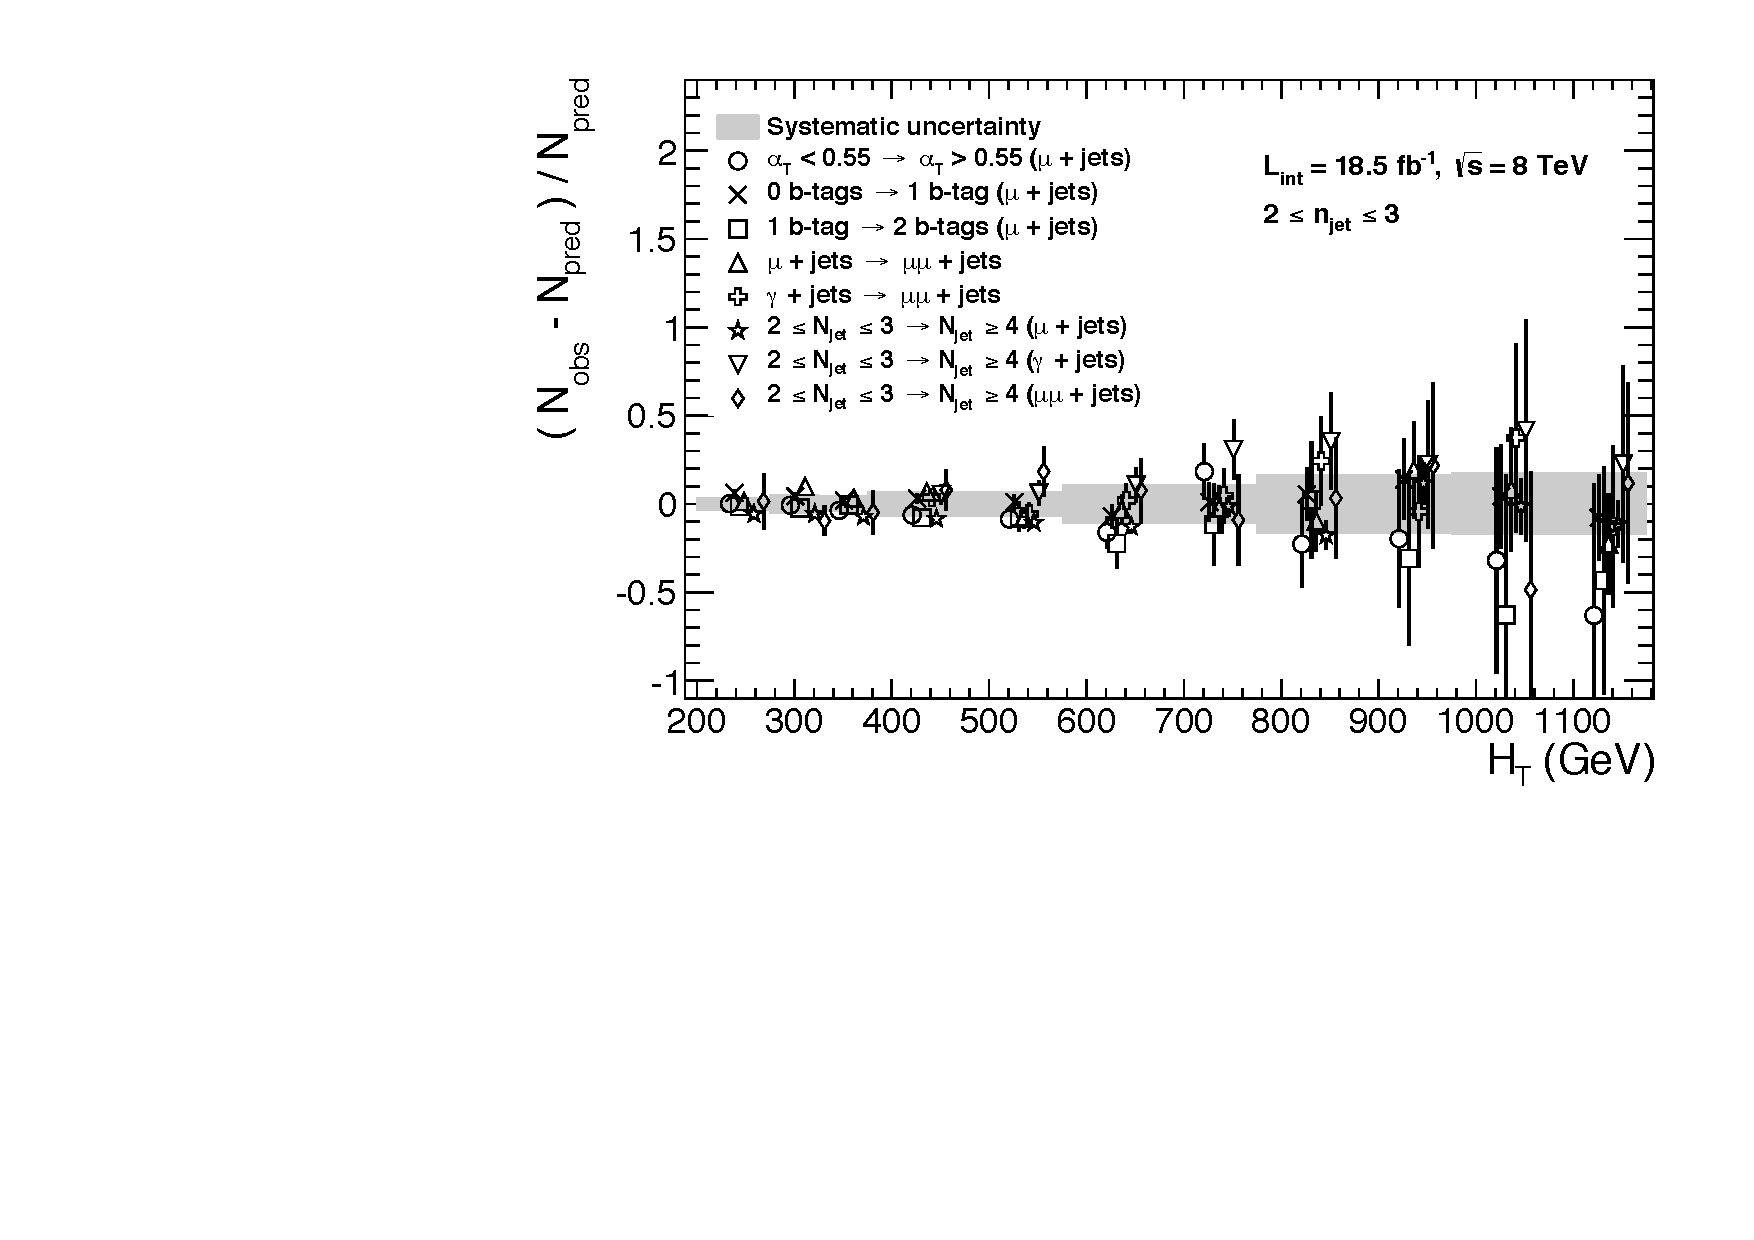
\includegraphics[width=\textwidth]{Figs/syst/v0/le3j/summary_plot}
    \caption{$2 \leq \nj \leq 3$}
    \label{fig:closure_summary_le3j}
  \end{subfigure}             
  \begin{subfigure}[b]{0.7\textwidth}
    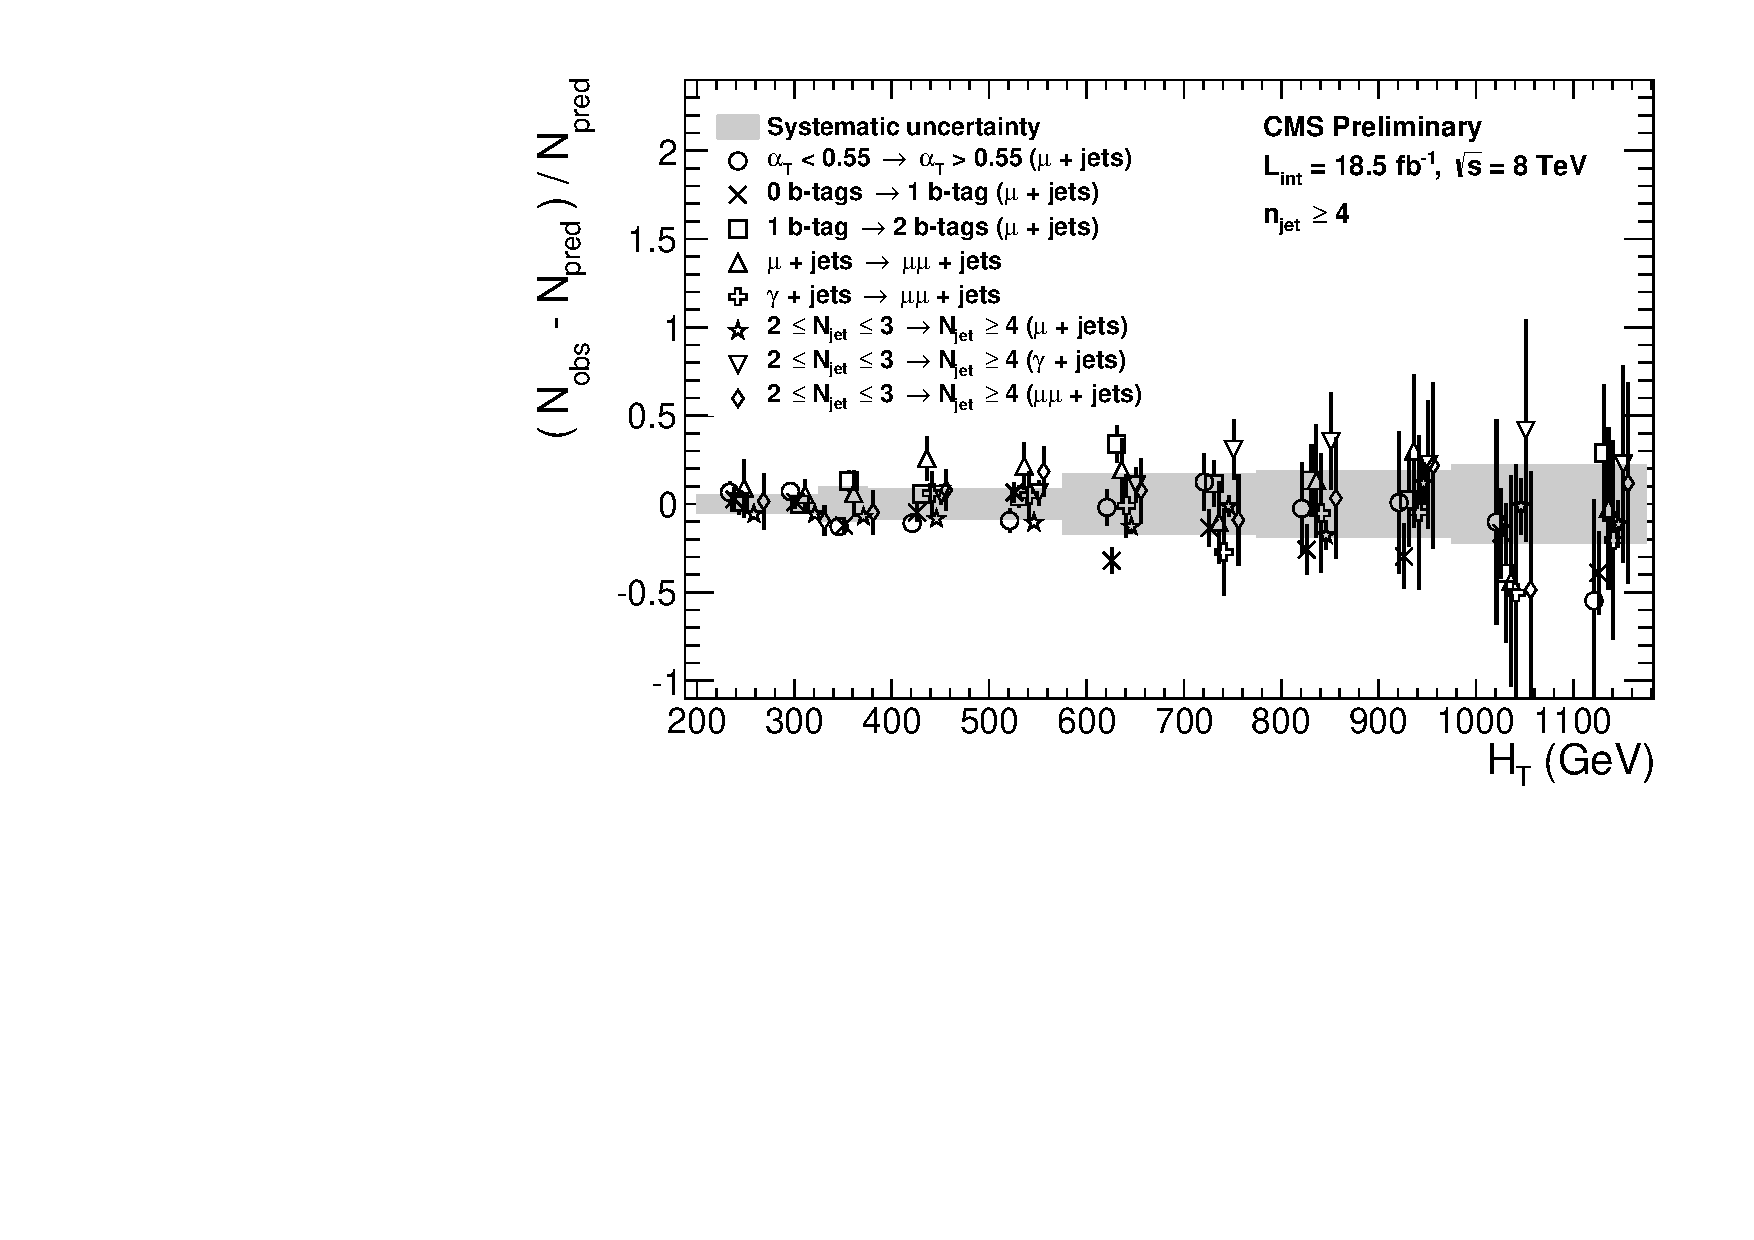
\includegraphics[width=\textwidth]{Figs/syst/v0/ge4j/summary_plot}
    \caption{$\nj \geq 4$}
    \label{fig:closure_summary_ge4j}
  \end{subfigure}             
  \caption{Sets of closure tests (open symbols) overlaid on top of
      the systematic uncertainty used for each of the five \HT
      regions (shaded bands) and for the two different jet
      multiplicity bins: (a) $2 \leq \nj \leq 3$ and (b) $\nj \geq
      4$. REWORD}
  \label{fig:closure_summary}
\end{figure}

Figure~\ref{fig:closure_summary} shows a summary of eight of the closure tests 
considered as `core' tests for the analysis, split into both
\njlow (figure~\ref{fig:closure_summary_le3j}) 
and \njhigh (figure~\ref{fig:closure_summary_ge4j}).

The first test, represented by open circles, tests the modelling of the \alphat 
variable in the \mj control sample. In the analysis a prediction is made 
between the \mj control sample, which has no \alphat requirement, and the 
signal region, which has a tight \alphat requirement. This particular test 
probes
the validity of predicting between the `bulk' distribution of the control sample
and the `tail' distribution in the signal region. A similar test is also made 
in the \mmj control sample.

The next two tests, represented by crosses and open squares, test between 
different b-tag multiplicities in the \mj control sample. The different b-tag 
requirements greatly change the relative admixture of \wj (0b) and \ttj (1b) events. 
Given the focus on b-tagging, this test also investigates the simulations 
modelling of b-quark jets. It is important to note that this test is 
considered conservative, given that the admixture of \wj to \ttj events 
varies minimally between control and signal regions, where this extrapolation is 
made in the analysis.

A similar test is made for the relative admixture of \zj to \wj and \ttj, by 
predicting between the \mj and \mmj control regions. Again, this is considered 
conservative, but also probes the muon reconstruction and trigger efficiencies 
between the different muon multiplicities. These are however already well 
studied with data-driven techniques by the muon POG.

As described in section~\ref{sec:background_overview}, the \zinv prediction 
comes both the \gj and \mmj samples, and so a test is constructed to 
predict between these two orthogonal control regions, as shown by the open 
triangles.

The final three tests, indicated by open stars, triangles and diamonds, make 
predictions between the two different jet multiplicity categories, thereby 
testing the jet reconstruction and modelling. This test is also considered very 
conservative as the analysis only predicts between identical \nj categories in 
the control and signal regions.

The summary plots of these eight tests shown in figure~\ref{fig:closure_summary} 
indicate that there is no stastically significant biases or \HT dependencies. 
Figures~\ref{fig:closure_fit_le3j_pol0} and \ref{fig:closure_fit_ge4j_pol0} show
zeroeth order polynominal fit (blue lines) is made to each individual test to assess the 
level of any potential bias present. In addition, a first order polynominal fit 
(red lines) is 
also made to assess any potential \HT dependence present in the tests.
The best-fit values, $\chi^2$ and $p$-values 
obtained from both fits are summarised for each \nj category in
tables~\ref{tab:syst-fits-le3j}, \ref{tab:syst-fits-ge4j} and
\ref{tab:syst-fits-njet}.

As expected, the fits show no significant biases or trends, and therefore 
indicate good closure. The only exception is the 0 b-jets \ra 1 b-jet (\mj) test
for the \njhigh category
which showed a sub-optimal goodness of fit value. After investigation this was 
attributed to an upwards and downwards fluctuation in the 475-575 \gev and 575-
675 \gev bins respectively. Also shown in table~\ref{tab:syst-fits-ge4j} is the 
same fit made when summing these two bins - a fit which returns significantly 
improved fit values. This leads to the conclusion that these two bins contian a 
statistical fluctuation as opposed to a systematic bias.

could go into more detail describing the outcomes of the fits...

\begin{figure}[ht!]
  \centering
  \begin{subfigure}[b]{0.46\textwidth}
    \includegraphics[width=\textwidth]{figures/syst/v0/le3j/summary_plot_pol0}
    \caption{$2 \leq \nj \leq 3$ (zeroeth order polynomial fits)}
    \label{fig:closure_fit_le3j_pol0}
  \end{subfigure}
  \begin{subfigure}[b]{0.46\textwidth}
    \includegraphics[width=\textwidth]{figures/syst/v0/le3j/summary_plot_pol1}
    \caption{$2 \leq \nj \leq 3$ (first order polynomial fits)}
    \label{fig:closure_fit_le3j_pol1}
  \end{subfigure}
  \begin{subfigure}[b]{0.46\textwidth}
    \includegraphics[width=\textwidth]{figures/syst/v0/ge4j/summary_plot_pol0}
    \caption{$\nj \geq 4$ (zeroeth order polynomial fits)}
    \label{fig:closure_fit_ge4j_pol0}
  \end{subfigure}
  \begin{subfigure}[b]{0.46\textwidth}
    \includegraphics[width=\textwidth]{figures/syst/v0/ge4j/summary_plot_pol1}
    \caption{$\nj \geq 4$ (first order polynomial fits)}
    \label{fig:closure_fit_ge4j_pol1}
  \end{subfigure}
  \caption{Sets of closure tests (open symbols) overlaid on top of
      the systematic uncertainty used for each of the five \HT
      regions (shaded bands), for the two different jet multiplicity
      bins (top row) $2 \leq \nj \leq 3$ and (bottom row) $\nj
      \geq 4$, and with zeroeth (left column) and first (right column)
      order polynomial fits to each set of closure tests. REWORD}
  \label{fig:closure_fits}
\end{figure}

\begin{table}[!ht]
  \caption{A summary of the results obtained from fits of zeroeth
    order polynomials (i.e. a constant) to five sets of closure tests
    performed in the \njlow bin. The final two columns show the best
    fit value for the slope obtained when performing a linear fit and
    the $p$-value for the linear fit. REWORD}
  \label{tab:syst-fits-le3j}
  \centering
  \scriptsize
  \begin{tabular}{ llrccccrc }
    \hline
    \hline
                                              &          & \multicolumn{4}{c}{Constant fit} &          & \multicolumn{2}{c}{Linear fit}                        \\
    \cline{3-6}\cline{8-9}                                                                  
    Closure test                              & Symbol   & Best fit value                   & $\chi^2$ & d.o.f. & $p$-value &  & Slope ($10^{-4}$) & $p$-value \\
    \hline                                                                                                                                  
    $\alphat < 0.55 \ra \alphat > 0.55$ (\mj) & Circle   & $-0.02 \pm 0.01$                 & 11.3     & 10     & 0.34      &  & $-2.9 \pm 1.1$    & 0.83      \\ 
    0 b-jets \ra 1 b-jet (\mj)                & Times    & $ 0.04 \pm 0.01$                 & 5.8      & 10     & 0.83      &  & $-1.5 \pm 0.9$    & 0.97      \\ 
    1 b-jet \ra 2 b-jets (\mj)                & Square   & $-0.03 \pm 0.02$                 & 5.3      & 10     & 0.87      &  & $-3.0 \pm 1.7$    & 0.99      \\ 
    \mj \ra \mmj                              & Triangle & $ 0.03 \pm 0.02$                 & 12.3     & 10     & 0.27      &  & $-1.3 \pm 1.1$    & 0.28      \\ 
    \gj \ra \mmj                              & Cross    & $-0.02 \pm 0.03$                 & 3.0      & 7      & 0.88      &  & $ 0.0 \pm 2.7$    & 0.81      \\ 
    \hline
    \hline
  \end{tabular}
\end{table}

\begin{table}[!ht]
  \caption{A summary of the results obtained from fits of zeroeth
    order polynomials (i.e. a constant) to five sets of closure tests
    performed in the \njhigh bin. The final two columns show the best
    fit value for the slope obtained when performing a linear fit and
    the $p$-value for the linear fit. $^{\dag} $See text for details
    on this particular fit. REWORD} 
  \label{tab:syst-fits-ge4j}
  \centering
  \scriptsize
  \begin{tabular}{ llrccccrc }
    \hline
    \hline
                                              &          & \multicolumn{4}{c}{Constant fit} &          & \multicolumn{2}{c}{Linear fit}                        \\
    \cline{3-6}\cline{8-9}                                                                  
    Closure test                              & Symbol   & Best fit value                   & $\chi^2$ & d.o.f. & $p$-value &  & Slope ($10^{-4}$) & $p$-value \\
    \hline                                                                                                                                 
    $\alphat < 0.55 \ra \alphat > 0.55$ (\mj) & Circle   & $-0.02 \pm    0.02$              & 17.6     & 10     & 0.06      &  & $-3.1 \pm 1.7$    & 0.11      \\ 
    0 b-jets \ra 1 b-jet (\mj)                & Times    & $-0.06 \pm 0.02$                 & 31.2     & 10     & 0.00      &  & $-4.1 \pm 1.2$    & 0.02      \\ 
    0 b-jets \ra 1 b-jet (\mj)$^{ \dag}$      & Times    & $-0.05 \pm 0.02$                 & 13.4     & 9      & 0.15      &  & $-3.9 \pm 1.3$    & 0.78      \\ 
    1 b-jet \ra 2 b-jets (\mj)                & Square   & $ 0.06 \pm    0.02$              & 13.7     & 10     & 0.19      &  & $ 2.5 \pm 1.6$    & 0.28      \\ 
    \mj \ra \mmj                              & Triangle & $ 0.11 \pm    0.05$              & 4.8      & 10     & 0.90      &  & $ 0.4 \pm 2.7$    & 0.85      \\ 
    \gj \ra \mmj                              & Cross    & $-0.00 \pm 0.07$                 & 2.3      & 7      & 0.94      &  & $-5.3 \pm 4.7$    & 0.99      \\ 
    \hline
    \hline
  \end{tabular}
\end{table}

\begin{table}[!ht]
  \caption{A summary of the results obtained from fits of zeroeth
    order polynomials (i.e. a constant) to three sets of closure tests
    (\njlow \ra \njhigh) that probe the accuracy of the MC
    modelling of the \nj distribution observed in data, using the
    three data control samples.  REWORD} 
  \label{tab:syst-fits-njet}
  \centering
  \footnotesize
  \begin{tabular}{ llrccccrc }
    \hline
    \hline
           &                   & \multicolumn{4}{c}{Constant fit} &          & \multicolumn{2}{c}{Linear fit}                        \\
    \cline{3-6}\cline{8-9}
    Sample & Symbol            & Best fit value                   & $\chi^2$ & d.o.f. & $p$-value &  & Slope ($10^{-4}$) & $p$-value \\
    \hline                                                                                                            
    \mj    & Star              & $-0.08 \pm 0.01$                 & 9.3      & 10     & 0.50      &  & $0.6 \pm 0.7$     & 0.48      \\ 
    \gj    & Inverted triangle & $ 0.09 \pm 0.04$                 & 3.7      & 7      & 0.82      &  & $5.1 \pm 3.2$     & 0.98      \\ 
    \mmj   & Diamond           & $-0.00 \pm 0.05$                 & 4.7      & 10     & 0.91      &  & $2.5 \pm 2.9$     & 0.92      \\ 
    \hline
    \hline
  \end{tabular}
\end{table}

Maybe also include a couple other relevant tests.

may also include SITV closure tests


\subsection{Background uncertainty summary}
Under the assumption of closure for the eight core tests, as determined in the 
previous section, systematic errors are assigned in seven regions of \HT, for 
each \nj category.

Values are calculated by summing in quadrature the weighted mean and sample 
variance for all eight tests in a given \HT region. These values are summarised 
in table~\ref{tab:syst_values} and also in the summary plots of figure~\ref{fig:closure_summary},
shown as grey bands.

\begin{table}[!ht]
  \caption{A summary of the magnitude of the systematic uncertainties (\%)
    assigned to the transfer factors, according to \nj and \HT
    region. REWORD}
  \label{tab:syst_values}
  \centering
  \footnotesize
  \begin{tabular}{ cccccccc }
    \hline
    \hline
            & \multicolumn{7}{c}{\HT region (GeV)}                                \\
    \cline{2-8}
    \nj   & 200--275 & 275--325 & 325--375 & 375--575 & 575--775 & 775-975 & $>975$ \\
    \hline                                                                                                                                  
    2--3    & 4        & 6        & 6        & 8        & 12       & 17      & 19     \\
    $\geq$4 & 6        & 6        & 11       & 11       & 18       & 20      & 26     \\
    \hline                                                                                                                                  
    \hline
  \end{tabular}
\end{table}

Systematic values are here considered as fully uncorrelated between the 
different analysis categories and the \HT regions defined here, which is again 
considered as a conservative approach given that some correlation is to be 
expected between adjacent \HT bins, for example.
